\documentclass[../main.tex]{subfiles}

\begin{document}

\section*{Chapter 10}
\addcontentsline{toc}{section}{Chapter 10}

%
\subsection*{Example 10.1*}
\addcontentsline{toc}{subsection}{Exercise 10.1*}
%
Binary system acetonitrile(1)/nitromethane(2) conforms closely to Raoult's law.
Vapor pressures for the pure species are given by the following
Antoine equations:
%
\begin{gather*}% opts
  \ln P_1^{\text{sat}} / \unit{kPa} = 14.2724 - \frac{2945.47}{T - 49.15}\\
  \ln P_2^{\text{sat}} / \unit{kPa} = 14.2043 - \frac{2972.64}{T - 64.15}
\end{gather*}
%
\begin{enumerate}[label=(\alph*)]
  \item Prepare a graph showing $P$ vs. $x_{1}$ and $P$ vs. $y_{1}$
    for a temperature of 75~\unit{\degreeCelsius}.
  \item Prepare graph showing $t$ vs. $x_{1}$ and $t$ vs. $y_{2}$
    for a pressure of 70~\unit{\kilo\pascal}.
\end{enumerate}
%
\begin{solution}% opts
  %
  \begin{enumerate}[label=(\alph*)]
    \item
      %
      \begin{gather*}% opts
        P_{\alpha} = x_{\alpha}P_{\alpha}^{*}\\
        \intertext{Substitute this to the Antoine equation:}
        \ln{\frac{P_{\alpha}/\unit{\kilo\pascal}}{x_{\alpha}}} = A_{\alpha} -
        \frac{B_{\alpha}}{t/\unit{\degreeCelsius}+C_{\alpha}}\\
        P = P_{1}^{\text{sat}}x_{1} + P_{2}^{\text{sat}}(1-x_{1})\\
        y_{\alpha} = \frac{P_{\alpha}}{P} =
        \frac{P_{\alpha}^{\text{sat}}x_{\alpha}}{P}
      \end{gather*}
      The plot is shown in Figure~(\ref{fig:e10-1a})
      %
      \begin{figure}[h!]
        \centering
        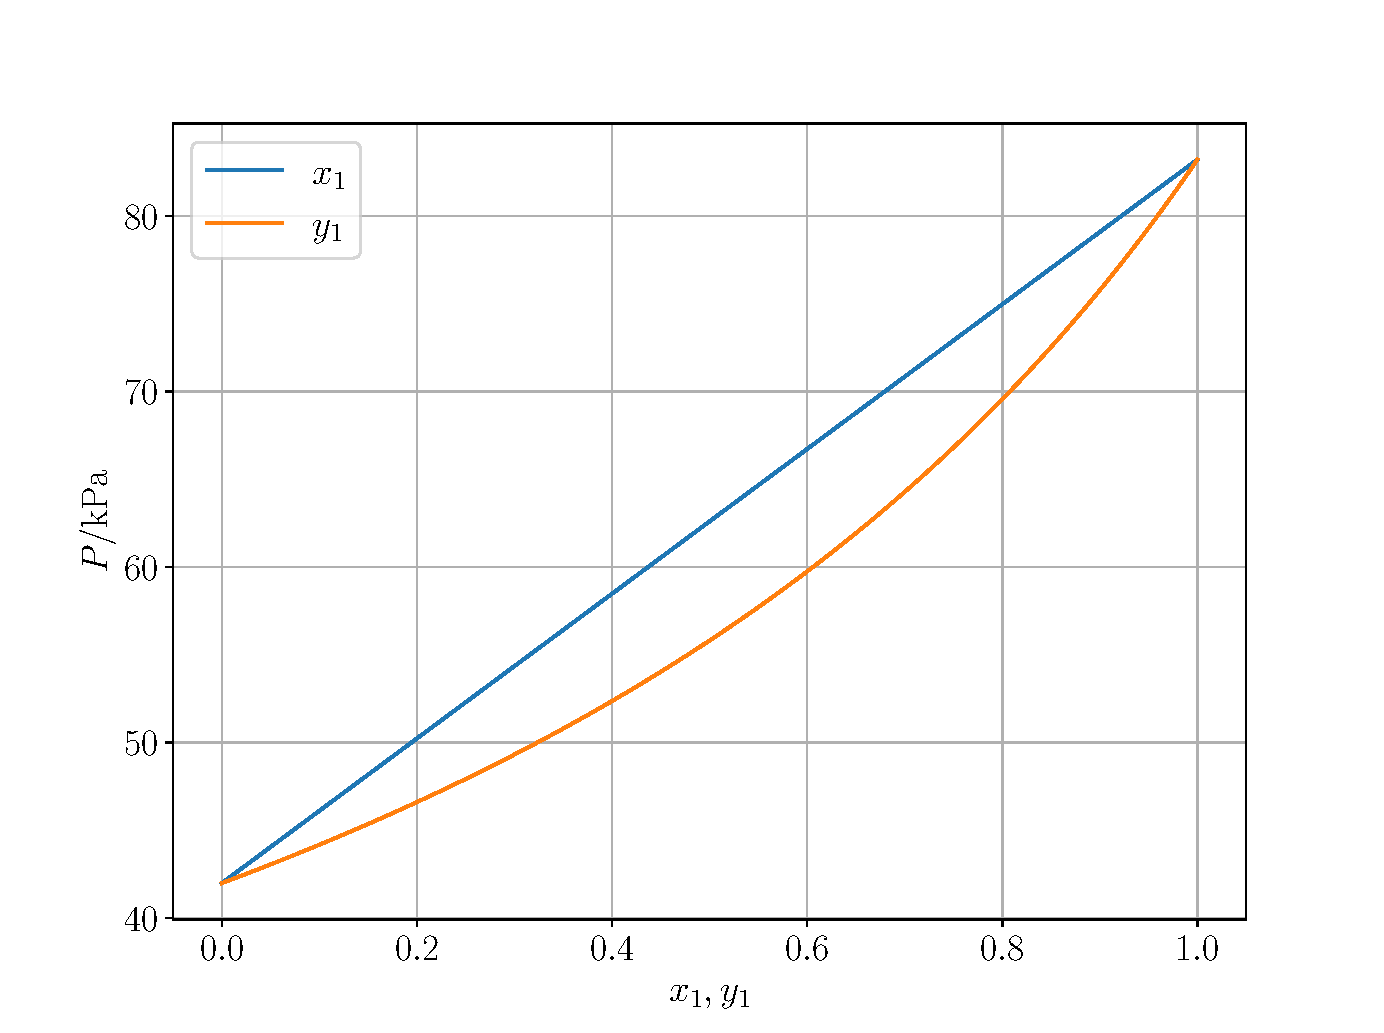
\includegraphics[scale=0.5]{../img/e10-1.pdf}%
        \caption{Plot of pressure versus liquid and vapor mole fraction
        of component 1 as described in Example 10.1a*}
        \label{fig:e10-1a}
      \end{figure}
      %
    \item
      This is another form of the Antoine equation:
      %
      \begin{gather*}% opts
        T_{\alpha}^{\text{sat}} = \frac{B_{\alpha}}{A_{\alpha} - \ln
        P} + C_{\alpha}\\
        \intertext{Solve for $T_{1}^{\text{sat}}$ and
          $T_{2}^{\text{sat}}$ as these comprise of the range of the graph. %
          Solve for:
        }
        \ln P_{\alpha}^{\text{sat}} = A_{\alpha} -
        \frac{B_{\alpha}}{T+C_{\alpha}}\\
        \intertext{To solve for:}
        x_{1}=\frac{P-P_{2}^{\text{sat}}}{P_{1}^{\text{sat}}-P_{2}^{\text{sat}}}\\
        \intertext{Which is derived from:}
        P = P_{1}^{\text{sat}}x_{1} + P_{2}^{\text{sat}}(1-x_{1})
      \end{gather*}
      %
      The plot is shown in Figure~(\ref{fig:e10-1b})
      \begin{figure}[h!]
        \centering
        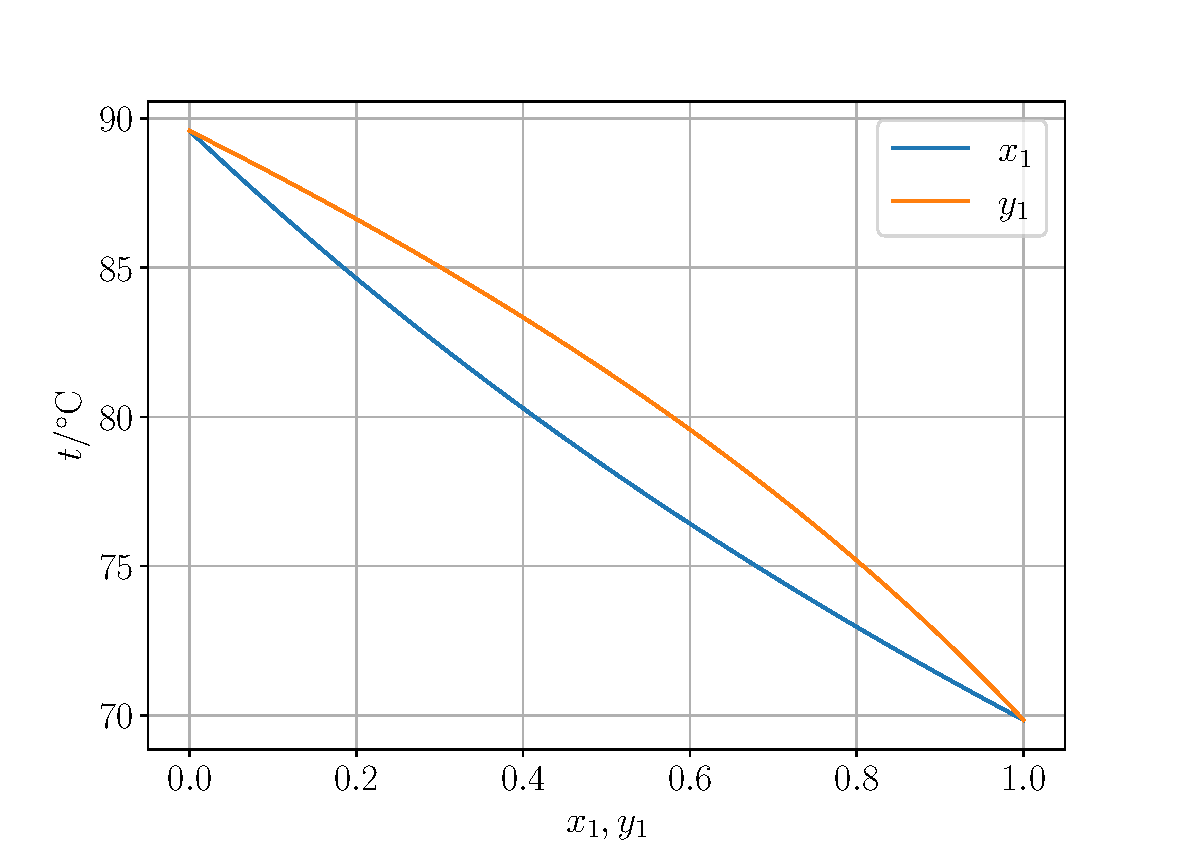
\includegraphics[scale=0.6]{../img/e10-1b.pdf}%
        \caption{Plot of temperature (in \unit{\degreeCelsius})
          versus liquid and vapor mole fraction of component 1 as
          described in Example 10.1b*
        }
        \label{fig:e10-1b}
      \end{figure}
      %
  \end{enumerate}
  %
\end{solution}

%
\subsection*{Example 10.2*}
\addcontentsline{toc}{subsection}{Example 10.2*}
%
Assuming that carbonated water contains only $\ce{CO2}$(1) and
$\ce{H2O}$(2), determine the compositions of the vapor and liquid
phases in a sealed can of "soda" and the pressure exerted on the can
at 10~\unit{\degreeCelsius} (283.15~\unit{\kelvin}). Henry's constant
for $\ce{CO2}$ in water at 10~\unit{\degreeCelsius}
(283.15~\unit{\kelvin}) is about 990~\unit{\bar}
%
\begin{solution}% opts
  Applying the phase rule:
  %
  \begin{gather*}% opts
    F = 2 - \pi + N \\
    F = 2
  \end{gather*}
  %
  Only the temperature of the system is given. We must give another
  intensive variable. And since we are given the Henry's constant it
  is good that we limit the amount of $\ce{C02}$ in the liquid, $x_{1}=0.01$.
  %
  \begin{gather*}% opts
    y_{1}P = x_{1}\mathcal{H}_{1} \qquad y_{2}P = x_{2}P_{2}^{\text{sat}}\\
    P = x_{1}\mathcal{H}_{1} + x_{2}P_{2}^{\text{sat}}
  \end{gather*}
  %
  The value of $P_{2}\text{sat}$ can be found at the steam table, at
  10~\unit{\degreeCelsius}, which is 0.01227~\unit{\bar}
  \begin{gather*}% opts
    P = (0.01)(990) + (0.99)(0.01227) = \boxed{9.912~\unit{\bar}}\\
    y_{2} = \frac{x_{2}P_{2}^{\text{sat}}}{P} =
    \frac{(0.99)(0.01227)}{9.912} = \boxed{0.0012}\\
    y_{1} = \boxed{0.9988}
  \end{gather*}
\end{solution}
%

%
\subsection*{Example 10.3*}
\addcontentsline{toc}{subsection}{Example 10.3*}
%
For the system methanol(1)/methyl acetate(2), the following equations
provide a reasonable correlation for the activity coefficients"
\begin{gather*}% opts
  \ln y_{1} = Ax_{2}^{2} \qquad \ln y_{2} = Ax_{1}^{2} \\
  \text{where } A = 2.771 - 0.00523 T
\end{gather*}
In addition, the following Antoine equations provide vapor pressures:
\begin{gather*}% opts
  \ln P_{1}^{\text{sat}} = 16.59158 - \frac{3643.31}{T - 33.424} \\
  \ln P_{2}^{\text{sat}} = 14.25326 - \frac{2665.54}{T - 53.424}
\end{gather*}
where T is in kelvins and the vapor pressures are in kPa. Assuming
the validity of Eq~(\ref{eq:mrl}), calculate
%
\begin{enumerate}[label=(\alph*)]
  \item $P$ and $\{y_{i}\}$, for $t/T =
    45~\unit{\degreeCelsius}/318.15~\unit{\kelvin}$ and $x_{1}=0.25$
  \item $P$ and $\{x_{i}\}$, for $t/T =
    45~\unit{\degreeCelsius}/318.15~\unit{\kelvin}$ and $y_{1}=0.60$
  \item $T$ and $\{y_{i}\}$, for $P = 101.33~\unit{\kilo\pascal}$ and
    $x_{1}=0.85$
  \item $T$ and $\{x_{i}\}$, for $P = 101.33~\unit{\kilo\pascal}$ and
    $y_{1}=0.40$
  \item The azeotropic pressure, and the azeotropic composition, for
    $t/T = 45~\unit{\degreeCelsius}/318.15~\unit{\kelvin}$
\end{enumerate}
%
\begin{equation*}% opts
  y_{i}P = x_{i}\gamma_{i}P_{i}^{\text{sat}} \qquad (i = 1,2,\dots,N)
  \label{eq:mrl}
\end{equation*}
%
\begin{solution}% opts
  %
  \begin{enumerate}[label=(\alph*)]
    \item
      Solve for the activity coefficients:
      \begin{gather*}% opts
        A = 2.771 - (0.00523)(318.15) = 1.107\\
        \gamma_{1} = \exp{(Ax_{2}^{2})} = 1.864\\
        \gamma_{2} = \exp{(Ax_{1}^{2})} = 1.072
      \end{gather*}
      And then for pressure:
      \begin{gather*}% opts
        P = x_{1}\gamma_{1}P_{1}^{\text{sat}} +
        x_{2}\gamma_{2}P_{2}^{\text{sat}}\\
        P = \boxed{73.50~\unit{\kilo\pascal}}
      \end{gather*}
      And then for the vapor mole fractions:
      \begin{gather*}% opts
        y_{i} = x_{i}\gamma_{i}P_{i}^{\text{sat}}/P
      \end{gather*}
      \begin{empheq}[box=\widefbox]{gather*}
        y_{1} = 0.281\\
        y_{2} = 0.719
      \end{empheq}
    \item Figure~(\ref{fig:e10-3b}) shows the diagram of the
      iteration solution to be used.
      %
      \begin{figure}[h!]
        \centering
        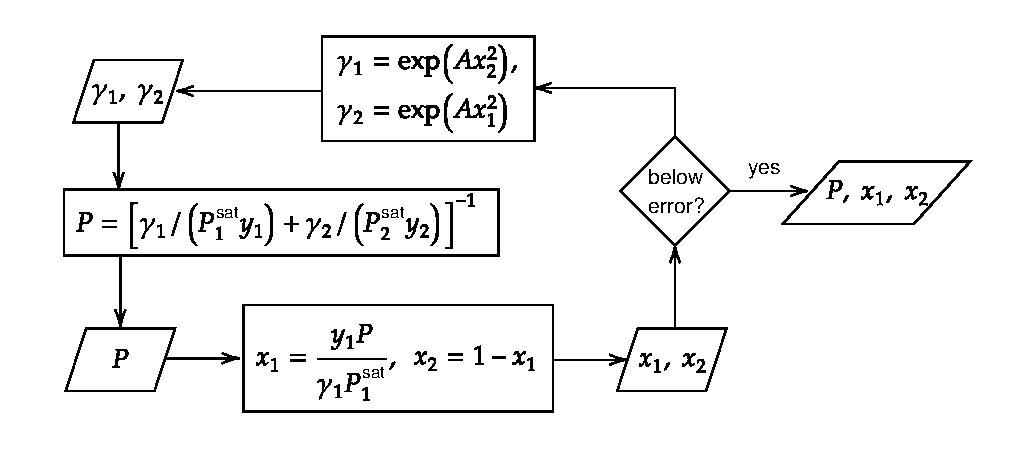
\includegraphics[width=\linewidth]{../img/e10-3b.pdf}%
        \caption{A schematic diagram for the iteration method to be
        used for Example 10.3b.}
        \label{fig:e10-3b}
      \end{figure}
      %
      The initial guesses are $\gamma_{1}=1$ and $\gamma_{2}=1$.
      After the 12th iteration, the error is less than $1\times10^{-6}$.
      \begin{empheq}[box=\widefbox]{gather*}
        P = 62.63~\unit{\kilo\pascal}\\
        x_{1} = 0.82\\
        x_{2} = 0.18
      \end{empheq}
    \item
      \begin{gather*}% opts
        T_{i}^{\text{sat}} = \frac{B_{i}}{A_{i} - \ln P} - C_{i} \\
        T_{1}^{\text{sat}} = 337.71~\unit{\kelvin} \\
        T_{2}^{\text{sat}} = 330.08~\unit{\kelvin} \\
        \intertext{A mole-fraction-weighted average of these values
        then provides an initial $T$ for the iteration:}
        T = x_{1}T_{1} + x_{2}T_{2} \\
        T = 336.57~\unit{\kelvin}
      \end{gather*}
      Solve for either $P_{1}^{\text{sat}}$ or $P_{2}^{\text{sat}}$
      and then solve for a new value of $T$. Using this $T$, solve
      for $A$, $\gamma_{1}$, and $\gamma_{2}$. The iteration method
      is shown as a schematic diagram in Figure~(\ref{fig:e10-3c})
      %
      \begin{figure}[h!]
        \centering
        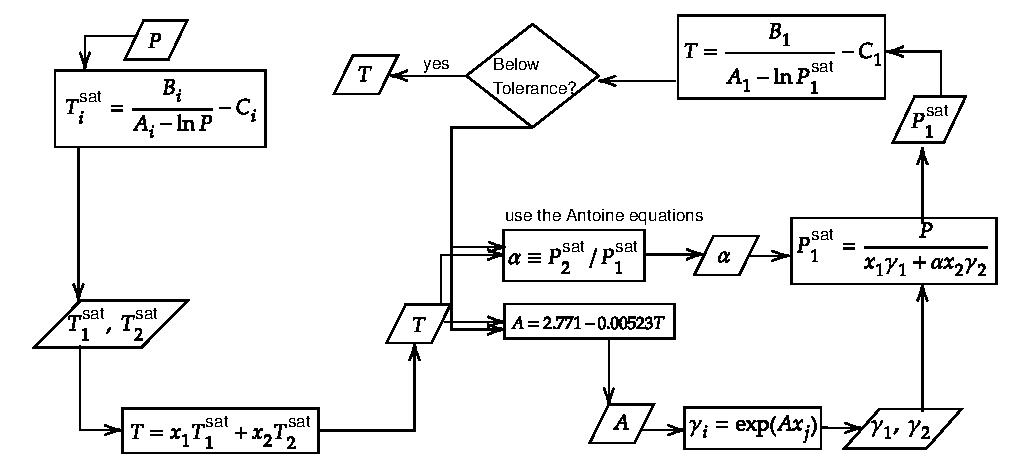
\includegraphics[width=\linewidth]{../img/e10-3c.pdf}%
        \caption{A schematic diagram showing the iteration method
        used in 10.3c.}
        \label{fig:e10-3c}
      \end{figure}
      %
      \begin{empheq}[box=\widefbox]{gather*}
        T = 255.45~\unit{\kelvin} \\
        x_{1} = 0.4633 \\
        x_{2} = 0.5367
      \end{empheq}
    \item
      The iteration method to be done is shown in Figure~(\ref{fig:e10-3d})
      %
      \begin{figure}[h!]
        \centering
        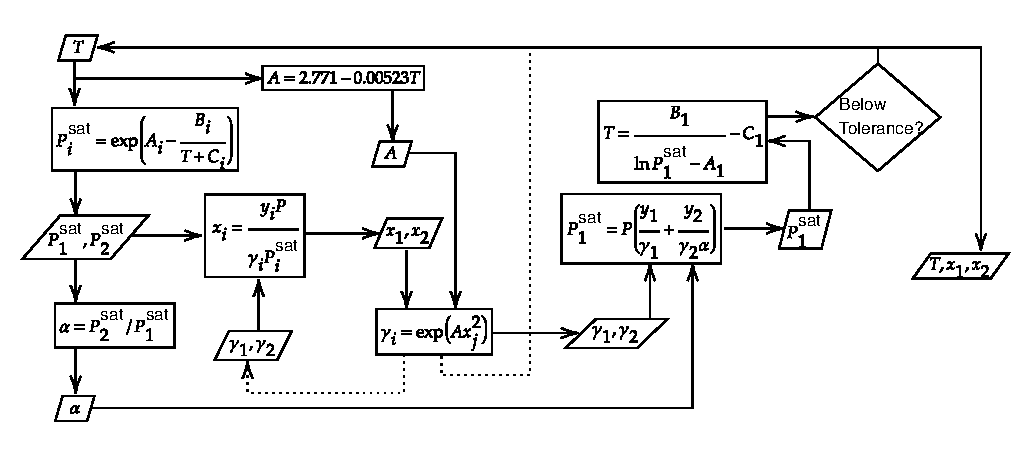
\includegraphics[width=\linewidth]{../img/e10-3d.pdf}%
        \caption{A schematic diagram showing the iteration method
        used in 10.3d.}
        \label{fig:e10-3d}
      \end{figure}
      %

  \end{enumerate}
  %
\end{solution}
%

%
\subsection*{Example 10.4*}
\addcontentsline{toc}{subsection}{Example 10.4*}
% DI TO KASAMA

%
\subsection*{Example 10.5*}
\addcontentsline{toc}{subsection}{Example 10.5*}
%
The system acetone(1)/acetonitrile(2)/nitromethane(3) at
80~\unit{\degreeCelsius} and 100~\unit{\kilo\pascal} has the overall
composition, $z_{1}=0.45$, $z_{2}=0.35$, $z_{3}=0.20$. Assuming that
Raoult's law is appropriate to this system, determine $\mathcal{L}$,
$\mathcal{V}$, $\{x_{i}\}$, $\{y_{i}\}$. The vapor pressures of the
pure species at 80~\unit{\degreeCelsius} are:
%
\begin{gather*}% opts
  P_1^{\text{sat}} = 195.75 \qquad P_2^{\text{sat}} = 97.84 \qquad
  P_3^{\text{sat}} = 50.32~\unit{\kilo\Pascal}
\end{gather*}
%
%
\begin{solution}% opts
  %
  \begin{gather*}% opts
    x_{i} = \frac{z_{i}}{1 + (V/F)(K_{i}-1)}\\
    1 = \frac{z_{1}}{1 + (V/F)(K_{1}-1)} + \frac{z_{2}}{1 +
    (V/F)(K_{2}-1)} + \frac{z_{3}}{1 + (V/F)(K_{3} - 1 )}\\
    K_{i} = \frac{P_{i}^{\text{sat}}}{P}\\
  \end{gather*}
  %
\end{solution}
%

%
\subsection*{Problem 10.1}
\addcontentsline{toc}{subsection}{Problem 10.1}
%
Assuming the validity of Raoult's law, do the following calculations
for the benzene(1)/toluene(2) system:
%
\begin{enumerate}[label=(\alph*)]
  \item Given $x_{1} = 0.33$ and $T=100~\unit{\degreeCelsius}$, find
    $y_{1}$ and $P$.
  \item Given $y_{1} = 0.33$ and $T=100~\unit{\degreeCelsius}$, find
    $x_{1}$ and $P$.
  \item Given $x_{1} = 0.33$ and $P=120~\unit{\kilo\pascal}$, find
    $y_{1}$ and $T$.
  \item Given $y_{1} = 0.33$ and $P=120~\unit{\kilo\pascal}$, find
    $x_{1}$ and $T$.
  \item Given $T=105~\unit{\degreeCelsius}$ and
    $P=120~\unit{\kilo\pascal}$ find $x_{1}$ and $y_{1}$.
  \item For part (e), if the \textit{overall} mole fraction of
    benzene is $z_{1}=0.33$, what molar fraction of the two-phase
    system is vapor?
  \item Why is Raoult's law likely to be an excellent VLE model for
    this system at the stated (or computed) conditions?
\end{enumerate}
%
\begin{solution}% opts
  \begin{align*}% opts
    A_{1} = 13.7819 & \qquad A_{2} = 13.9320 \\
    B_{1} = 2726.81 & \qquad B_{2} = 3056.96 \\
    C_{1} = 217.572 & \qquad C_{2} = 217.625
  \end{align*}
  %
  \begin{enumerate}[label=(\alph*)]

    \item $x_{1}=0.33$ and $T=100~\unit{\degreeCelsius}$, find $P$ and $y_{1}$
      \begin{gather*}% opts
        \ln P_{i}^{\text{sat}}/\unit{\kilo\pascal} = A_{i} -
        \frac{B_{i}}{t/\unit{\degreeCelsius} + C_{i}} \\
        P_{1}^{\text{sat}} = 180.45~\unit{\kilo\pascal} \\
        P_{2}^{\text{sat}} = 74.26~\unit{\kilo\pascal} \\
        P = P_{1}^{\text{sat}}x_{1} + P_{2}^{\text{sat}}(1-x_{1}) \\
        \boxed{P=109.30~\unit{\kilo\pascal}} \\
        y_{1} = \frac{x_{1}P_{1}^{\text{sat}}}{P} \\
        \boxed{y_{1} = 0.5448}
      \end{gather*}

    \item $y_{1}=0.33$ and $T=100~\unit{\degreeCelsius}$, find $x_{1}$ and $P$
      \begin{gather*}% opts
        x_{1} = \frac{y_{1}P}{P_{1}^{\text{sat}}} \\
        P = y_{1}P + P_{2}^{\text{sat}}\left(1 -
        \frac{y_{1}P}{P_{1}^{\text{sat}}}\right)
      \end{gather*}
      \begin{empheq}[box=\widefbox]{gather*}
        P = 92.156~\unit{\kilo\pascal} \\
        x_{1} = 0.169
      \end{empheq}

    \item $x_{1}=0.33$ and $P=120~\unit{\kilo\pascal}$, find $y_{1}$ and $T$
      \begin{gather*}% opts
        x_{1}\cdot\exp\left(A_{1} - \frac{B_{1}}{T + C_{1}}\right) +
        x_{2}\cdot\exp\left(A_{2} - \frac{B_{2}}{T + C_{2}}\right) = P \\
        P_{1}^{\text{sat}} = A_{1} - \frac{B_{1}}{T + C_{1}} \\
        y_{1} = \frac{x_{1}P_{1}^{\text{sat}}}{P}
      \end{gather*}
      \begin{empheq}[box=\widefbox]{gather*}
        T = 103.307~\unit{\degreeCelsius} \\
        y_{1} = 0.542
      \end{empheq}

    \item $y_{1}=0.33$ and $P=120~\unit{\kilo\pascal}$, find $x_{1}$ and $T$
      \begin{gather*}% opts
        P = x_{1}P_{1}^{\text{sat}} + (1-x_{1})P_{2}^{\text{sat}} \\
        x_{1} = \frac{y_{1}P}{P_{1}^{\text{sat}}}
        P = y_{1}P + (1 -
        \frac{y_{1}P}{P_{1}^{\text{sat}}})P_{2}^{\text{sat}} \\
        P_{i}^{\text{sat}} = A_{i} - \frac{B_{i}}{T + C_{i}}
      \end{gather*}
      \begin{empheq}[box=\widefbox]{gather*}
        T = 109.13~\unit{\degreeCelsius} \\
        x_{1} = 0.1726
      \end{empheq}

    \item $T = 105~\unit{\degreeCelsius}$, $P =
      120~\unit{\kilo\pascal}$, find $x_{1}$, $y_{1}$
      \begin{gather*}% opts
        P = y_{1}P + \left(1 -
        \frac{y_{1}P}{P_{1}^{\text{sat}}}\right)P_{2}^{\text{sat}} \\
        P_{i}^{\text{sat}} = A_{i} - \frac{B_{i}}{T + C_{i}} \\
        x_{i} = \frac{y_{i}P}{P_{i}^{\text{sat}}}
      \end{gather*}
      \begin{empheq}[box=\widefbox]{gather*}
        y_{1} = 0.4840 \\
        x_{1} = 0.2818
      \end{empheq}

    \item $z_{1}=0.33$, find $\mathcal{V}$
      \begin{gather*}% opts
        z_{1} = \frac{\mathcal{L}x_{1} +
        \mathcal{V}y_{1}}{\mathcal{L} + \mathcal{V}}
        \intertext{Basis: $\mathcal{L} + \mathcal{V} = 1~\unit{\mole}$}
        z_{1} = \mathcal{L}x_{1} + (1 -
        \mathcal{L})y_{1} \\
        \mathcal{L} = 0.7616 \\
        \boxed{V = 0.2384}
      \end{gather*}

    \item Benzene and toluene are two very similar compounds on top
      of being non-polar, minimizing chemical interactions.

  \end{enumerate}
  %
\end{solution}

\end{document}
